\documentclass[aps,superscriptaddress,notitlepage]{revtex4-1}

\usepackage{amsmath,amsfonts,amssymb,graphicx,hyperref,listings,xcolor,float}
\usepackage[ddmmyyyy,24hr]{datetime}

\definecolor{purple}{HTML}{CC78BC}
\definecolor{green}{HTML}{029E73}
\definecolor{blue}{HTML}{0173B2}
\definecolor{lightblue}{HTML}{56B4E9}
\definecolor{yellow}{HTML}{DE8F05}
\definecolor{brown}{HTML}{CA9161}
\definecolor{red}{HTML}{D55E00}
\definecolor{grey}{HTML}{949494}
\definecolor{pink}{HTML}{FBAFE4}
\definecolor{lightyellow}{HTML}{ECE133}

\usepackage{tikz}
\usetikzlibrary{calc}
\usetikzlibrary{arrows.meta,arrows}
\def\scale{0.8}

\begin{document}

%%%%% TITLE

\title{(Active) vertex model}
\author{Yann-Edwin Keta}
\date{\today, \currenttime}
\maketitle

%%%%% CONTENT

\section{Mesh}

\begin{figure}[H]
\centering
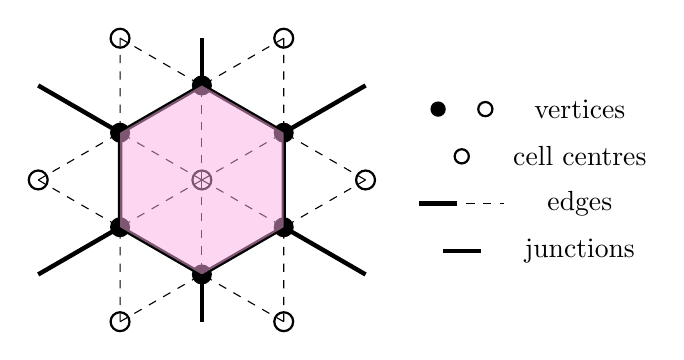
\begin{tikzpicture}[scale=0.75*\scale]

% FIRST CELL
% cell centre
\coordinate (A) at (0, 0);
\draw[thick] (A) circle (0.2);
% cell corners
\coordinate (B) at ($(A) + ({2*cos(30 + 0*60)}, {2*sin(30 + 0*60)})$);
\draw[fill=black] (B) circle (0.2);
\coordinate (C) at ($(A) + ({2*cos(30 + 1*60)}, {2*sin(30 + 1*60)})$);
\draw[fill=black] (C) circle (0.2);
\coordinate (D) at ($(A) + ({2*cos(30 + 2*60)}, {2*sin(30 + 2*60)})$);
\draw[fill=black] (D) circle (0.2);
\coordinate (E) at ($(A) + ({2*cos(30 + 3*60)}, {2*sin(30 + 3*60)})$);
\draw[fill=black] (E) circle (0.2);
\coordinate (F) at ($(A) + ({2*cos(30 + 4*60)}, {2*sin(30 + 4*60)})$);
\draw[fill=black] (F) circle (0.2);
\coordinate (G) at ($(A) + ({2*cos(30 + 5*60)}, {2*sin(30 + 5*60)})$);
\draw[fill=black] (G) circle (0.2);
% junctions
\draw[ultra thick] (B) -- (C) -- (D) -- (E) -- (F) -- (G) -- (B);
% inner edges
\draw[dashed] (A) -- (B);
\draw[dashed] (A) -- (C);
\draw[dashed] (A) -- (D);
\draw[dashed] (A) -- (E);
\draw[dashed] (A) -- (F);
\draw[dashed] (A) -- (G);
% fill
\fill[opacity=0.5, pink] (B) -- (C) -- (D) -- (E) -- (F) -- (G) -- (B);

% SECOND CELL
% cell centre
\coordinate (H) at ($(B) + ({2*cos(30)}, {-2*sin(30)})$);
\draw[thick] (H) circle (0.2);
% cell corners
\coordinate (I) at ($(H) + (0, 2)$);
\coordinate (J) at ($(H) + (0, -2)$);
% juntions
\draw[ultra thick] (B) -- (I);
\draw[ultra thick] (G) -- (J);
% inner edges
\draw[dashed] (H) -- (B);
\draw[dashed] (H) -- (G);

% THIRD CELL
% cell centre
\coordinate (K) at ($(D) + ({-2*cos(30)}, {-2*sin(30)})$);
\draw[thick] (K) circle (0.2);
% cell corners
\coordinate (L) at ($(K) + (0, 2)$);
\coordinate (M) at ($(K) + (0, -2)$);
% juntions
\draw[ultra thick] (D) -- (L);
\draw[ultra thick] (E) -- (M);
% inner edges
\draw[dashed] (K) -- (D);
\draw[dashed] (K) -- (E);

% ADDITIONAL POINTS
\coordinate (N) at ($(C) + (0, 1)$);
\draw[ultra thick] (C) -- (N);
\coordinate (O) at ($(F) + (0, -1)$);
\draw[ultra thick] (F) -- (O);

% ADDITIONAL CELL CENTRES
% cell centre
\coordinate (P) at ($(B) + (0, 2)$);
\draw[thick] (P) circle (0.2);
% inner edges
\draw[dashed] (P) -- (B);
\draw[dashed] (P) -- (C);
% cell centre
\coordinate (Q) at ($(D) + (0, 2)$);
\draw[thick] (Q) circle (0.2);
% inner edges
\draw[dashed] (Q) -- (C);
\draw[dashed] (Q) -- (D);
% cell centre
\coordinate (R) at ($(E) + (0, -2)$);
\draw[thick] (R) circle (0.2);
% inner edges
\draw[dashed] (R) -- (E);
\draw[dashed] (R) -- (F);
% cell centre
\coordinate (S) at ($(G) + (0, -2)$);
\draw[thick] (S) circle (0.2);
% inner edges
\draw[dashed] (S) -- (F);
\draw[dashed] (S) -- (G);

% LEGEND
\draw[fill=black] (5, 1.5) circle (0.15);
\draw[thick] (6, 1.5) circle (0.15);
\draw (8, 1.5) node[]{vertices};
\draw[thick] (5.5, 0.5) circle (0.15);
\draw (8, 0.5) node[]{cell centres};
\draw[ultra thick] (4.6, -0.5) -- ++(0.8, 0);
\draw[dashed] (5.6, -0.5) -- ++(0.8, 0);
\draw (8, -0.5) node[]{edges};
\draw[ultra thick] (5.1, -1.5) -- ++ (0.8, 0);
\draw (8, -1.5) node[]{junctions};

\end{tikzpicture}
\caption{Schematic of a cell (highlighted in pink) in the vertex model. A \textit{cell centre} is enclosed by \textit{cell corners} (or \textit{vertices}). These are linked between themselves by \textit{junctions}.}
\end{figure}

We will assume (i) that cells are always convex so that the mesh remains planar, and (ii) that no edge joins two cell centres. The ensemble of the vertices and the edges that link them constitutes the \textit{geometric mesh}. The specification of the cell centres and the junctions between non-cell-centres defines the \textit{physical mesh}.

\section{Cell potential energy}

\begin{figure}[H]
\centering
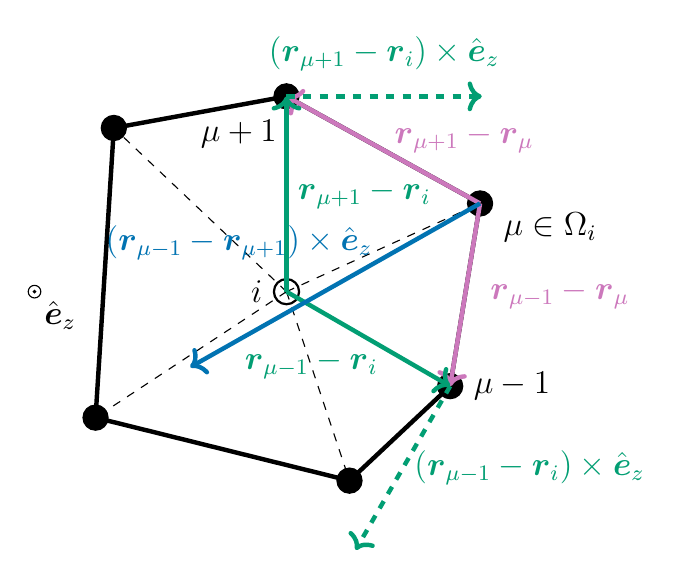
\begin{tikzpicture}[scale=\scale]

% FIRST CELL
% cell centre
\coordinate (A) at (0, 0);
\draw[thick] (A) circle (0.2) node[left,xshift=-5pt]{\large $i$};
% cell corners
\coordinate (B) at ($(A) + ({4*cos(30 + 0.2*60) + 0.1}, {3*sin(30 + 0*60) - 0.1})$);
\draw[fill=black] (B) circle (0.2) node[below right,xshift=5pt]{\large $\mu \in \Omega_i$};
\coordinate (C) at ($(A) + ({2.9*cos(30 + 1*60)}, {3.1*sin(30 + 1*60)})$);
\draw[fill=black] (C) circle (0.2) node[below left,yshift=-5pt]{\large $\mu + 1$};
\coordinate (D) at ($(A) + ({3*cos(30 + 2.1*60)}, {3*sin(30 + 1.5*60)})$);
\draw[fill=black] (D) circle (0.2);
\coordinate (E) at ($(A) + ({3.5*cos(30 + 3*60)}, {4*sin(30 + 3*60)})$);
\draw[fill=black] (E) circle (0.2);
\coordinate (F) at ($(A) + ({1 + 3*cos(30 + 4*60)}, {3*sin(30 + 4*60)})$);
\draw[fill=black] (F) circle (0.2);
\coordinate (G) at ($(A) + ({3*cos(30 + 5*60)}, {3*sin(30 + 5*60)})$);
\draw[fill=black] (G) circle (0.2) node[right,xshift=5pt]{\large $\mu - 1$};
% junctions
\draw[ultra thick] (B) -- (C) -- (D) -- (E) -- (F) -- (G) -- (B);
% inner edges
\draw[dashed] (A) -- (B);
\draw[dashed] (A) -- (C);
\draw[dashed] (A) -- (D);
\draw[dashed] (A) -- (E);
\draw[dashed] (A) -- (F);
\draw[dashed] (A) -- (G);

\draw (-4, 0) circle (0.1) node[below right]{\large $\hat{\boldsymbol{e}}_z$};
\draw[fill=black] (-4, 0) circle (0.02);

% perimeter term
\draw[purple, ultra thick, ->] (B) -- (C) node[midway, above right, xshift=0pt, yshift=-5pt]{\large $\boldsymbol{r}_{\mu + 1} - \boldsymbol{r}_{\mu}$};
\draw[purple, ultra thick, ->] (B) -- (G) node[midway, right, xshift=5pt]{\large $\boldsymbol{r}_{\mu - 1} - \boldsymbol{r}_{\mu}$};

% area term
\draw[green, ultra thick, ->] (A) -- (C) node[midway, right]{\large $\boldsymbol{r}_{\mu + 1} - \boldsymbol{r}_i$};
\draw[green, ultra thick, ->] (A) -- (G) node[midway, below left, xshift=7.5pt]{\large $\boldsymbol{r}_{\mu - 1} - \boldsymbol{r}_i$};
% https://tex.stackexchange.com/a/63569
\draw[green, ultra thick, dashed, ->] let \p{A}=(A), \p{C}=(C) in (C) -- ++({\y{C} - \y{A}}, {-(\x{C} - \x{A})}) node[midway, above, yshift=5pt]{\large $(\boldsymbol{r}_{\mu + 1} - \boldsymbol{r}_i) \times \hat{\boldsymbol{e}}_z$};
\draw[green, ultra thick, dashed, ->] let \p{A}=(A), \p{G}=(G) in (G) -- ++({\y{G} - \y{A}}, {-(\x{G} - \x{A})}) node[midway, right, yshift=0pt]{\large $(\boldsymbol{r}_{\mu - 1} - \boldsymbol{r}_i) \times \hat{\boldsymbol{e}}_z$};
\draw[blue, ultra thick, ->] let \p{C}=(C), \p{G}=(G) in (B) -- ++({-(\y{C} - \y{G})}, {(\x{C} - \x{G})}) node[midway, above left, xshift=17.5pt, yshift=5pt]{\large $(\boldsymbol{r}_{\mu - 1} - \boldsymbol{r}_{\mu + 1}) \times \hat{\boldsymbol{e}}_z$};

\end{tikzpicture}
\caption{Vertex representation of a single cell. By convention, cell centres are denoted by latin indices, and cell corners are denotes by greek indices. We denote $\Omega_i$ the ensemble of cell corners $\mu$ of the cell whose centre is $i$. By convention, $\mu + 1$ (respectively $\mu - 1$) denotes the next cell corner of $i$ after $\mu$ in anticlockwise (respectively clockwise) order.}
\label{fig:fmu}
\end{figure}

We introduce for each cell $i$ a reference perimeter $P^0_i$ and a reference area $A^0_i$, and for each of its cell corner $\mu \in \Omega_i$ a force whose effect is to bring the cell's perimeter $P_i$ and area $A_i$ to their reference quantities. A possible force derives from the following potential energy \cite{farhadifar2007influence,fletcher2014vertex,sknepnek2023generating}
\begin{equation}
E_{\mathrm{VM}} = \sum_{\text{cells } i} \left[\frac{1}{2} K_i (A_i - A_i^0)^2 + \frac{1}{2} \Gamma_i (P_i - P_i^0)^2\right],
\label{eq:evm}
\end{equation}
where $K_i$ and $\Gamma_i$ are respectively area and perimeter elastic constants. We denote $\boldsymbol{r}_{\mu}$, $\boldsymbol{r}_i$ the position of vertices $\mu, i$. The cell's perimeter can be written
\begin{equation}
P_i = \sum_{\mu \in \Omega_i} |\boldsymbol{r}_{\mu} - \boldsymbol{r}_{\mu - 1}|,
\end{equation}
and the cell's area can be computed with the shoelace formula
\begin{equation}
A_i = \sum_{\mu \in \Omega_i} \frac{1}{2} [(\boldsymbol{r}_{\mu} - \boldsymbol{r}_{i}) \times (\boldsymbol{r}_{\mu - 1} - \boldsymbol{r}_{i})] \cdot \hat{\boldsymbol{e}}_z.
\end{equation}
Note that, by convention of ordering of cell corners, each term in this sum \textit{must be} positive. With these notations, we thus write the force acting on vertex $\mu$
\begin{equation}
\boldsymbol{F}_{\mathrm{VM},\mu} = -\nabla_{\mu} E_{\mathrm{VM}},
\label{eq:fmugrade}
\end{equation}
where $\nabla_{\mu} \equiv \partial/\partial \boldsymbol{r}_{\mu}$. We compute
\begin{equation}
\nabla_{\mu} \left(|\boldsymbol{r}_{\mu} - \boldsymbol{r}_{\mu - 1}|\right) = \frac{\boldsymbol{r}_{\mu} - \boldsymbol{r}_{\mu - 1}}{|\boldsymbol{r}_{\mu} - \boldsymbol{r}_{\mu - 1}|},
\end{equation}
as well as
\begin{equation}
\nabla_{\mu} \left([(\boldsymbol{r}_{\mu} - \boldsymbol{r}_i) \times (\boldsymbol{r}_{\mu - 1} - \boldsymbol{r}_i)] \cdot \hat{\boldsymbol{e}}_z\right) = (\boldsymbol{r}_{\mu - 1} - \boldsymbol{r}_i) \times \hat{\boldsymbol{e}}_z
\end{equation}
to write \eqref{eq:fmugrade} in its full form
\begin{equation}
\begin{aligned}
\boldsymbol{F}_{\mathrm{VM},\mu} &= - \sum_{\text{cells i},~ \mu \in \Omega_i} \bigg[\frac{1}{2} K_i (A_i - A^0_i) \left[(\boldsymbol{r}_{\mu + 1} - \boldsymbol{r}_i) \times \hat{\boldsymbol{e}}_z - (\boldsymbol{r}_{\mu - 1} - \boldsymbol{r}_i) \times \hat{\boldsymbol{e}}_z\right]\\
&\qquad\qquad\qquad\qquad+ \Gamma_i (P_i - P^0_i) \left[\frac{\boldsymbol{r}_{\mu} - \boldsymbol{r}_{\mu - 1}}{|\boldsymbol{r}_{\mu} - \boldsymbol{r}_{\mu - 1}|} + \frac{\boldsymbol{r}_{\mu} - \boldsymbol{r}_{\mu - 1}}{|\boldsymbol{r}_{\mu} - \boldsymbol{r}_{\mu - 1}|}\right]\bigg]\\
&= \sum_{\text{cells i},~ \mu \in \Omega_i} \bigg[\frac{1}{2} K_i (A_i - A^0_i) {\color{blue} \underbrace{(\boldsymbol{r}_{\mu - 1} - \boldsymbol{r}_{\mu + 1}) \times \hat{\boldsymbol{e}}_z}_{\text{towards cell interior}}} + \Gamma_i (P_i - P^0_i) \bigg[{\color{purple} \underbrace{\frac{\boldsymbol{r}_{\mu - 1} - \boldsymbol{r}_{\mu}}{|\boldsymbol{r}_{\mu - 1} - \boldsymbol{r}_{\mu}|}}_{\text{towards neighbour}}} + {\color{purple} \underbrace{\frac{\boldsymbol{r}_{\mu + 1} - \boldsymbol{r}_{\mu}}{|\boldsymbol{r}_{\mu + 1} - \boldsymbol{r}_{\mu}|}}_{\text{towards neighbour}}}\bigg]\bigg],
\end{aligned}
\end{equation}
where underbraced vectors are represented in Fig.~\ref{fig:fmu}. It is noteworthy that, with potential \eqref{eq:evm}, the force acting on each cell centre is zero
\begin{equation}
\boldsymbol{F}_{\mathrm{VM}, i} = - \nabla_i E_{\mathrm{VM}} = - \frac{1}{2} K_i (A_i - A^0_i) \sum_{\mu \in \Omega_i} (\boldsymbol{r}_{\mu} - \boldsymbol{r}_{\mu - 1}) \times \hat{\boldsymbol{e}}_z = 0.
\end{equation}

\section{Half-edge procedure}

\begin{figure}[H]
\centering
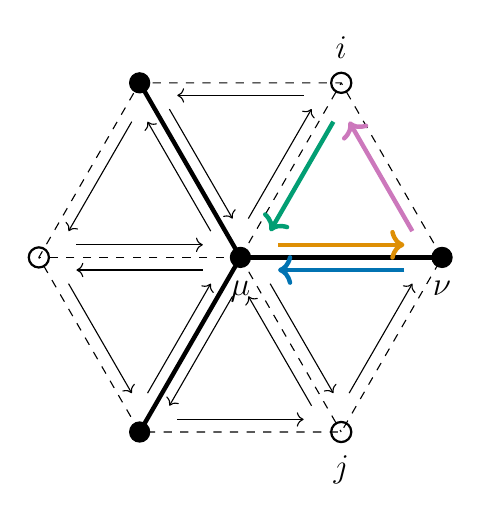
\begin{tikzpicture}[scale=0.8*\scale]

% vertices

\coordinate (A) at (0, 0);
\draw[fill=black] (A) circle (0.2) node[below, yshift=-5pt]{\large $\mu$};

\coordinate (B) at ($(A) + ({4*cos(0*60)}, {4*sin(0*60)})$);
\draw[fill=black] (B) circle (0.2) node[below, yshift=-5pt]{\large $\nu$};
\coordinate (C) at ($(A) + ({4*cos(1*60)}, {4*sin(1*60)})$);
\draw[thick] (C) circle (0.2) node[above, yshift=5pt]{\large $i$};
\coordinate (D) at ($(A) + ({4*cos(2*60)}, {4*sin(2*60)})$);
\draw[fill=black] (D) circle (0.2);
\coordinate (E) at ($(A) + ({4*cos(3*60)}, {4*sin(3*60)})$);
\draw[thick] (E) circle (0.2);
\coordinate (F) at ($(A) + ({4*cos(4*60)}, {4*sin(4*60)})$);
\draw[fill=black] (F) circle (0.2);
\coordinate (G) at ($(A) + ({4*cos(5*60)}, {4*sin(5*60)})$);
\draw[thick] (G) circle (0.2) node[below, yshift=-5pt]{\large $j$};

% edges

\draw[dashed] (B) -- (C) -- (D) -- (E) -- (F) -- (G) -- (B);

\draw[ultra thick] (A) -- (B);
\draw[dashed] (A) -- (C);
\draw[ultra thick] (A) -- (D);
\draw[dashed] (A) -- (E);
\draw[ultra thick] (A) -- (F);
\draw[dashed] (A) -- (G);

% intermediate points
\path (A) +({30 + 0*60}:0.5) coordinate (A0);
\path (A) +({30 + 1*60}:0.5) coordinate (A1);
\path (A) +({30 + 2*60}:0.5) coordinate (A2);
\path (A) +({30 + 3*60}:0.5) coordinate (A3);
\path (A) +({30 + 4*60}:0.5) coordinate (A4);
\path (A) +({30 + 5*60}:0.5) coordinate (A5);
\path (B) +({180 + 0*60 + 30}:0.5) coordinate (B0);
\path (B) +({180 + 0*60 - 30}:0.5) coordinate (B1);
\path (C) +({180 + 1*60 + 30}:0.5) coordinate (C0);
\path (C) +({180 + 1*60 - 30}:0.5) coordinate (C1);
\path (D) +({180 + 2*60 + 30}:0.5) coordinate (D0);
\path (D) +({180 + 2*60 - 30}:0.5) coordinate (D1);
\path (E) +({180 + 3*60 + 30}:0.5) coordinate (E0);
\path (E) +({180 + 3*60 - 30}:0.5) coordinate (E1);
\path (F) +({180 + 4*60 + 30}:0.5) coordinate (F0);
\path (F) +({180 + 4*60 - 30}:0.5) coordinate (F1);
\path (G) +({180 + 5*60 + 30}:0.5) coordinate (G0);
\path (G) +({180 + 5*60 - 30}:0.5) coordinate (G1);

% first triangle
\draw[ultra thick, yellow, ->] ($(A0)!0.1!(B1)$) -- ($(A0)!0.9!(B1)$);
\draw[ultra thick, purple, ->] ($(B1)!0.1!(C0)$) -- ($(B1)!0.9!(C0)$);
\draw[ultra thick, green, ->] ($(C0)!0.1!(A0)$) -- ($(C0)!0.9!(A0)$);
% second triangle
\draw[->] ($(A1)!0.1!(C1)$) -- ($(A1)!0.9!(C1)$);
\draw[->] ($(C1)!0.1!(D0)$) -- ($(C1)!0.9!(D0)$);
\draw[->] ($(D0)!0.1!(A1)$) -- ($(D0)!0.9!(A1)$);
% third triangle
\draw[->] ($(A2)!0.1!(D1)$) -- ($(A2)!0.9!(D1)$);
\draw[->] ($(D1)!0.1!(E0)$) -- ($(D1)!0.9!(E0)$);
\draw[->] ($(E0)!0.1!(A2)$) -- ($(E0)!0.9!(A2)$);
% fourth triangle
\draw[->] ($(A3)!0.1!(E1)$) -- ($(A3)!0.9!(E1)$);
\draw[->] ($(E1)!0.1!(F0)$) -- ($(E1)!0.9!(F0)$);
\draw[->] ($(F0)!0.1!(A3)$) -- ($(F0)!0.9!(A3)$);
% fifth triangle
\draw[->] ($(A4)!0.1!(F1)$) -- ($(A4)!0.9!(F1)$);
\draw[->] ($(F1)!0.1!(G0)$) -- ($(F1)!0.9!(G0)$);
\draw[->] ($(G0)!0.1!(A4)$) -- ($(G0)!0.9!(A4)$);
% sixth triangle
\draw[->] ($(A5)!0.1!(G1)$) -- ($(A5)!0.9!(G1)$);
\draw[->] ($(G1)!0.1!(B0)$) -- ($(G1)!0.9!(B0)$);
\draw[ultra thick, blue, ->] ($(B0)!0.1!(A5)$) -- ($(B0)!0.9!(A5)$);

\end{tikzpicture}
\caption{}
\end{figure}

\section{T1 transition}

\begin{figure}[H]
\centering
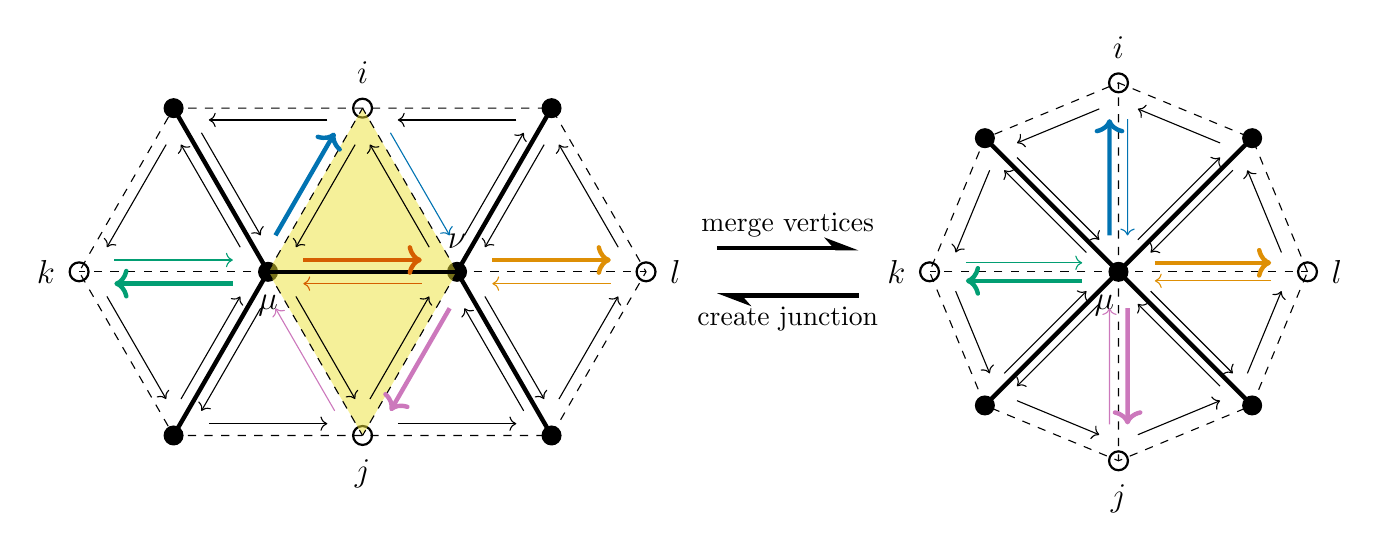
\begin{tikzpicture}[scale=0.75*\scale]

%%%%% BEFORE MERGE

% vertices

\coordinate (A) at (0, 0);
\draw[fill=black] (A) circle (0.2) node[below, yshift=-5pt]{\large $\mu$};

\coordinate (B) at ($(A) + ({4*cos(0*60)}, {4*sin(0*60)})$);
\draw[fill=black] (B) circle (0.2) node[above, yshift=5pt]{\large $\nu$};
\coordinate (C) at ($(A) + ({4*cos(1*60)}, {4*sin(1*60)})$);
\draw[thick] (C) circle (0.2) node[above, yshift=5pt]{\large $i$};
\coordinate (D) at ($(A) + ({4*cos(2*60)}, {4*sin(2*60)})$);
\draw[fill=black] (D) circle (0.2);
\coordinate (E) at ($(A) + ({4*cos(3*60)}, {4*sin(3*60)})$);
\draw[thick] (E) circle (0.2) node[left, xshift=-5pt]{\large $k$};
\coordinate (F) at ($(A) + ({4*cos(4*60)}, {4*sin(4*60)})$);
\draw[fill=black] (F) circle (0.2);
\coordinate (G) at ($(A) + ({4*cos(5*60)}, {4*sin(5*60)})$);
\draw[thick] (G) circle (0.2) node[below, yshift=-5pt]{\large $j$};
\coordinate (H) at ($(B) + ({4*cos(5*60)}, {4*sin(5*60)})$);
\draw[fill=black] (H) circle (0.2);
\coordinate (I) at ($(B) + ({4*cos(0*60)}, {4*sin(0*60)})$);
\draw[thick] (I) circle (0.2) node[right, xshift=5pt]{\large $l$};
\coordinate (J) at ($(B) + ({4*cos(1*60)}, {4*sin(1*60)})$);
\draw[fill=black] (J) circle (0.2);

\fill[opacity=0.5, lightyellow] (A) -- (G) -- (B) -- (C) -- (A);

% edges

\draw[dashed] (C) -- (D) -- (E) -- (F) -- (G) -- (H) -- (I) -- (J) -- (C);

\draw[ultra thick] (A) -- (B);
\draw[dashed] (A) -- (C);
\draw[ultra thick] (A) -- (D);
\draw[dashed] (A) -- (E);
\draw[ultra thick] (A) -- (F);
\draw[dashed] (A) -- (G);
\draw[dashed] (B) -- (G);
\draw[ultra thick] (B) -- (H);
\draw[dashed] (B) -- (I);
\draw[ultra thick] (B) -- (J);
\draw[dashed] (B) -- (C);

% intermediate points

\path (A) +({30 + 0*60}:0.5) coordinate (A0);
\path (A) +({30 + 1*60}:0.5) coordinate (A1);
\path (A) +({30 + 2*60}:0.5) coordinate (A2);
\path (A) +({30 + 3*60}:0.5) coordinate (A3);
\path (A) +({30 + 4*60}:0.5) coordinate (A4);
\path (A) +({30 + 5*60}:0.5) coordinate (A5);
\path (B) +({180 + 0*60 + 30}:0.5) coordinate (B0);
\path (B) +({180 + 0*60 - 30}:0.5) coordinate (B1);
\path (B) +({180 - 1*60 - 30}:0.5) coordinate (B2);
\path (B) +({180 - 2*60 - 30}:0.5) coordinate (B3);
\path (B) +({180 - 3*60 - 30}:0.5) coordinate (B4);
\path (B) +({180 - 4*60 - 30}:0.5) coordinate (B5);
\path (C) +({180 + 1*60 + 30}:0.5) coordinate (C0);
\path (C) +({180 + 1*60 - 30}:0.5) coordinate (C1);
\path (C) +({180 + 1*60 + 90}:0.5) coordinate (C5);
\path (D) +({180 + 2*60 + 30}:0.5) coordinate (D0);
\path (D) +({180 + 2*60 - 30}:0.5) coordinate (D1);
\path (E) +({180 + 3*60 + 30}:0.5) coordinate (E0);
\path (E) +({180 + 3*60 - 30}:0.5) coordinate (E1);
\path (F) +({180 + 4*60 + 30}:0.5) coordinate (F0);
\path (F) +({180 + 4*60 - 30}:0.5) coordinate (F1);
\path (G) +({180 + 5*60 + 30}:0.5) coordinate (G0);
\path (G) +({180 + 5*60 - 30}:0.5) coordinate (G1);
\path (G) +({180 + 5*60 - 90}:0.5) coordinate (G2);
\path (H) +({120 + 0*60 + 30}:0.5) coordinate (H0);
\path (H) +({120 + 0*60 - 30}:0.5) coordinate (H1);
\path (I) +({120 + 1*60 + 30}:0.5) coordinate (I0);
\path (I) +({120 + 1*60 - 30}:0.5) coordinate (I1);
\path (J) +({120 + 2*60 + 30}:0.5) coordinate (J0);
\path (J) +({120 + 2*60 - 30}:0.5) coordinate (J1);

% triangles

% first triangle
\draw[->, ultra thick, red] ($(A0)!0.1!(B1)$) -- ($(A0)!0.9!(B1)$);
\draw[->] ($(B1)!0.1!(C0)$) -- ($(B1)!0.9!(C0)$);
\draw[->] ($(C0)!0.1!(A0)$) -- ($(C0)!0.9!(A0)$);
% second triangle
\draw[->, ultra thick, blue] ($(A1)!0.1!(C1)$) -- ($(A1)!0.9!(C1)$);
\draw[->] ($(C1)!0.1!(D0)$) -- ($(C1)!0.9!(D0)$);
\draw[->] ($(D0)!0.1!(A1)$) -- ($(D0)!0.9!(A1)$);
% third triangle
\draw[->] ($(A2)!0.1!(D1)$) -- ($(A2)!0.9!(D1)$);
\draw[->] ($(D1)!0.1!(E0)$) -- ($(D1)!0.9!(E0)$);
\draw[->, green] ($(E0)!0.1!(A2)$) -- ($(E0)!0.9!(A2)$);
% fourth triangle
\draw[->, ultra thick, green] ($(A3)!0.1!(E1)$) -- ($(A3)!0.9!(E1)$);
\draw[->] ($(E1)!0.1!(F0)$) -- ($(E1)!0.9!(F0)$);
\draw[->] ($(F0)!0.1!(A3)$) -- ($(F0)!0.9!(A3)$);
% fifth triangle
\draw[->] ($(A4)!0.1!(F1)$) -- ($(A4)!0.9!(F1)$);
\draw[->] ($(F1)!0.1!(G0)$) -- ($(F1)!0.9!(G0)$);
\draw[->, purple] ($(G0)!0.1!(A4)$) -- ($(G0)!0.9!(A4)$);
% sixth triangle
\draw[->] ($(A5)!0.1!(G1)$) -- ($(A5)!0.9!(G1)$);
\draw[->] ($(G1)!0.1!(B0)$) -- ($(G1)!0.9!(B0)$);
\draw[->, red] ($(B0)!0.1!(A5)$) -- ($(B0)!0.9!(A5)$);
% seventh triangle
\draw[->, ultra thick, purple] ($(B5)!0.1!(G2)$) -- ($(B5)!0.9!(G2)$);
\draw[->] ($(G2)!0.1!(H0)$) -- ($(G2)!0.9!(H0)$);
\draw[->] ($(H0)!0.1!(B5)$) -- ($(H0)!0.9!(B5)$);
% eigth triangle
\draw[->] ($(B4)!0.1!(H1)$) -- ($(B4)!0.9!(H1)$);
\draw[->] ($(H1)!0.1!(I0)$) -- ($(H1)!0.9!(I0)$);
\draw[->, yellow] ($(I0)!0.1!(B4)$) -- ($(I0)!0.9!(B4)$);
% nineth triangle
\draw[->, ultra thick, yellow] ($(B3)!0.1!(I1)$) -- ($(B3)!0.9!(I1)$);
\draw[->] ($(I1)!0.1!(J0)$) -- ($(I1)!0.9!(J0)$);
\draw[->] ($(J0)!0.1!(B3)$) -- ($(J0)!0.9!(B3)$);
% tenth triangle
\draw[->] ($(B2)!0.1!(J1)$) -- ($(B2)!0.9!(J1)$);
\draw[->] ($(J1)!0.1!(C5)$) -- ($(J1)!0.9!(C5)$);
\draw[->, blue] ($(C5)!0.1!(B2)$) -- ($(C5)!0.9!(B2)$);

%%%%% ARROWS

\draw[ultra thick, arrows={-Stealth[harpoon]}] (9.5, 0.5) -- ++(3, 0) node[midway, above]{merge vertices};
\draw[ultra thick, arrows={-Stealth[harpoon]}] (12.5, -0.5) -- ++(-3, 0) node[midway, below]{create junction};

%%%%% AFTER MERGE

% vertices

\coordinate (A') at (18, 0);
\draw[fill=black] (A') circle (0.2) node[below left, xshift=2pt, yshift=-5pt]{\large $\mu$};

\coordinate (B') at ($(A') + ({4*cos(0*45)}, {4*sin(0*45)})$);
\draw[thick] (B') circle (0.2) node[right, xshift=5pt]{\large $l$};
\coordinate (C') at ($(A') + ({4*cos(1*45)}, {4*sin(1*45)})$);
\draw[fill=black] (C') circle (0.2);
\coordinate (D') at ($(A') + ({4*cos(2*45)}, {4*sin(2*45)})$);
\draw[thick] (D') circle (0.2) node[above, yshift=5pt]{\large $i$};
\coordinate (E') at ($(A') + ({4*cos(3*45)}, {4*sin(3*45)})$);
\draw[fill=black] (E') circle (0.2);
\coordinate (F') at ($(A') + ({4*cos(4*45)}, {4*sin(4*45)})$);
\draw[thick] (F') circle (0.2) node[left, xshift=-5pt]{\large $k$};
\coordinate (G') at ($(A') + ({4*cos(5*45)}, {4*sin(5*45)})$);
\draw[fill=black] (G') circle (0.2);
\coordinate (H') at ($(A') + ({4*cos(6*45)}, {4*sin(6*45)})$);
\draw[thick] (H') circle (0.2) node[below, yshift=-5pt]{\large $j$};
\coordinate (I') at ($(A') + ({4*cos(7*45)}, {4*sin(7*45)})$);
\draw[fill=black] (I') circle (0.2);

% edges

\draw[dashed] (B') -- (C') -- (D') -- (E') -- (F') -- (G') -- (H') -- (I') -- (B');

\draw[dashed] (A') -- (B');
\draw[ultra thick] (A') -- (C');
\draw[dashed] (A') -- (D');
\draw[ultra thick] (A') -- (E');
\draw[dashed] (A') -- (F');
\draw[ultra thick] (A') -- (G');
\draw[dashed] (A') -- (H');
\draw[ultra thick] (A') -- (I');

% intermediate points

\path (A') +({22.5 + 0*45}:0.5) coordinate (A'0);
\path (A') +({22.5 + 1*45}:0.5) coordinate (A'1);
\path (A') +({22.5 + 2*45}:0.5) coordinate (A'2);
\path (A') +({22.5 + 3*45}:0.5) coordinate (A'3);
\path (A') +({22.5 + 4*45}:0.5) coordinate (A'4);
\path (A') +({22.5 + 5*45}:0.5) coordinate (A'5);
\path (A') +({22.5 + 6*45}:0.5) coordinate (A'6);
\path (A') +({22.5 + 7*45}:0.5) coordinate (A'7);
\path (B') +({180 + 0*45 + 22.5}:0.5) coordinate (B'0);
\path (B') +({180 + 0*45 - 22.5}:0.5) coordinate (B'1);
\path (C') +({180 + 1*45 + 22.5}:0.5) coordinate (C'0);
\path (C') +({180 + 1*45 - 22.5}:0.5) coordinate (C'1);
\path (D') +({180 + 2*45 + 22.5}:0.5) coordinate (D'0);
\path (D') +({180 + 2*45 - 22.5}:0.5) coordinate (D'1);
\path (E') +({180 + 3*45 + 22.5}:0.5) coordinate (E'0);
\path (E') +({180 + 3*45 - 22.5}:0.5) coordinate (E'1);
\path (F') +({180 + 4*45 + 22.5}:0.5) coordinate (F'0);
\path (F') +({180 + 4*45 - 22.5}:0.5) coordinate (F'1);
\path (G') +({180 + 5*45 + 22.5}:0.5) coordinate (G'0);
\path (G') +({180 + 5*45 - 22.5}:0.5) coordinate (G'1);
\path (H') +({180 + 6*45 + 22.5}:0.5) coordinate (H'0);
\path (H') +({180 + 6*45 - 22.5}:0.5) coordinate (H'1);
\path (I') +({180 + 7*45 + 22.5}:0.5) coordinate (I'0);
\path (I') +({180 + 7*45 - 22.5}:0.5) coordinate (I'1);

% triangles

% first triangle
\draw[->, ultra thick, yellow] ($(A'0)!0.1!(B'1)$) -- ($(A'0)!0.9!(B'1)$);
\draw[->] ($(B'1)!0.1!(C'0)$) -- ($(B'1)!0.9!(C'0)$);
\draw[->] ($(C'0)!0.1!(A'0)$) -- ($(C'0)!0.9!(A'0)$);
% second triangle
\draw[->] ($(A'1)!0.1!(C'1)$) -- ($(A'1)!0.9!(C'1)$);
\draw[->] ($(C'1)!0.1!(D'0)$) -- ($(C'1)!0.9!(D'0)$);
\draw[->, blue] ($(D'0)!0.1!(A'1)$) -- ($(D'0)!0.9!(A'1)$);
% third triangle
\draw[->, ultra thick, blue] ($(A'2)!0.1!(D'1)$) -- ($(A'2)!0.9!(D'1)$);
\draw[->] ($(D'1)!0.1!(E'0)$) -- ($(D'1)!0.9!(E'0)$);
\draw[->] ($(E'0)!0.1!(A'2)$) -- ($(E'0)!0.9!(A'2)$);
% fourth triangle
\draw[->] ($(A'3)!0.1!(E'1)$) -- ($(A'3)!0.9!(E'1)$);
\draw[->] ($(E'1)!0.1!(F'0)$) -- ($(E'1)!0.9!(F'0)$);
\draw[->, green] ($(F'0)!0.1!(A'3)$) -- ($(F'0)!0.9!(A'3)$);
% fifth triangle
\draw[->, ultra thick, green] ($(A'4)!0.1!(F'1)$) -- ($(A'4)!0.9!(F'1)$);
\draw[->] ($(F'1)!0.1!(G'0)$) -- ($(F'1)!0.9!(G'0)$);
\draw[->] ($(G'0)!0.1!(A'4)$) -- ($(G'0)!0.9!(A'4)$);
% sixth triangle
\draw[->] ($(A'5)!0.1!(G'1)$) -- ($(A'5)!0.9!(G'1)$);
\draw[->] ($(G'1)!0.1!(H'0)$) -- ($(G'1)!0.9!(H'0)$);
\draw[->, purple] ($(H'0)!0.1!(A'5)$) -- ($(H'0)!0.9!(A'5)$);
% seventh triangle
\draw[->, ultra thick, purple] ($(A'6)!0.1!(H'1)$) -- ($(A'6)!0.9!(H'1)$);
\draw[->] ($(H'1)!0.1!(I'0)$) -- ($(H'1)!0.9!(I'0)$);
\draw[->] ($(I'0)!0.1!(A'6)$) -- ($(I'0)!0.9!(A'6)$);
% eighth triangle
\draw[->] ($(A'7)!0.1!(I'1)$) -- ($(A'7)!0.9!(I'1)$);
\draw[->] ($(I'1)!0.1!(B'0)$) -- ($(I'1)!0.9!(B'0)$);
\draw[->, yellow] ($(B'0)!0.1!(A'7)$) -- ($(B'0)!0.9!(A'7)$);

\end{tikzpicture}
\caption{}
\end{figure}

\begin{figure}[H]
\centering
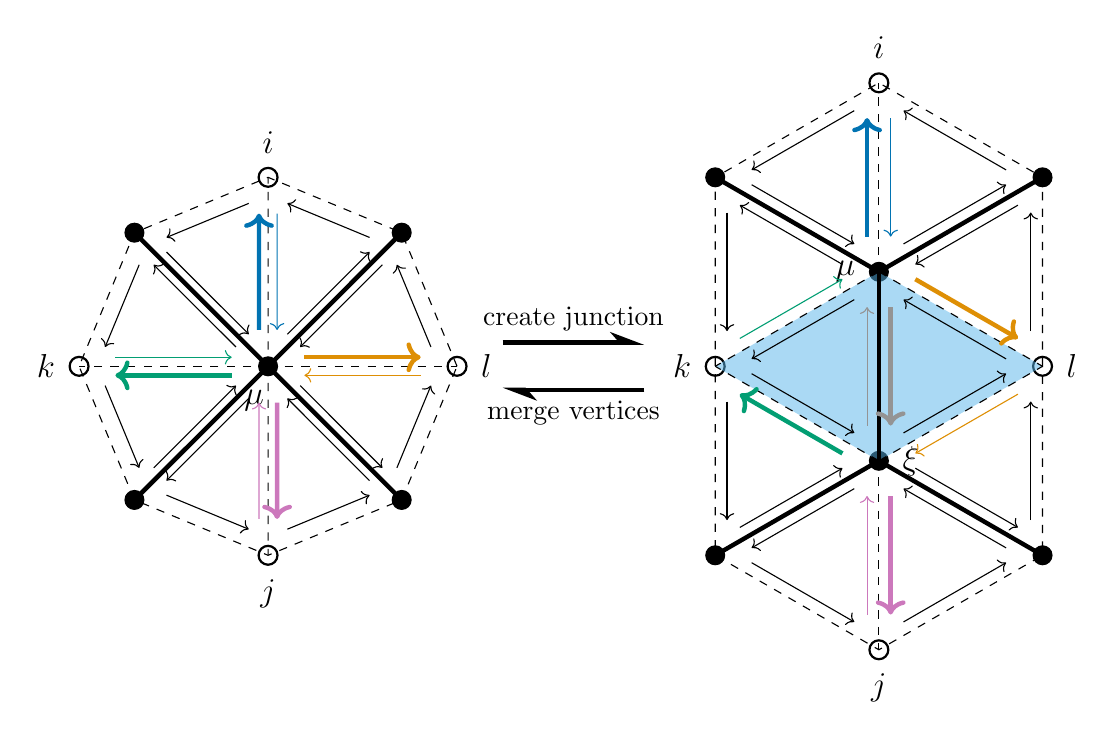
\begin{tikzpicture}[scale=0.75*\scale]

%%%%% BEFORE CREATION

% vertices

\coordinate (A) at (0, 2);
\draw[fill=black] (A) circle (0.2) node[left, xshift=-5pt]{\large $\mu$};

\coordinate (B) at ($(A) + ({4*cos(0*60 - 90)}, {4*sin(0*60 - 90)})$);
\draw[fill=black] (B) circle (0.2) node[right, xshift=5pt]{\large $\xi$};
\coordinate (C) at ($(A) + ({4*cos(1*60 - 90)}, {4*sin(1*60 - 90)})$);
\draw[thick] (C) circle (0.2) node[right, xshift=5pt]{\large $l$};
\coordinate (D) at ($(A) + ({4*cos(2*60 - 90)}, {4*sin(2*60 - 90)})$);
\draw[fill=black] (D) circle (0.2);
\coordinate (E) at ($(A) + ({4*cos(3*60 - 90)}, {4*sin(3*60 - 90)})$);
\draw[thick] (E) circle (0.2) node[above, yshift=5pt]{\large $i$};
\coordinate (F) at ($(A) + ({4*cos(4*60 - 90)}, {4*sin(4*60 - 90)})$);
\draw[fill=black] (F) circle (0.2);
\coordinate (G) at ($(A) + ({4*cos(5*60 - 90)}, {4*sin(5*60 - 90)})$);
\draw[thick] (G) circle (0.2) node[left, xshift=-5pt]{\large $k$};
\coordinate (H) at ($(B) + ({4*cos(5*60 - 90)}, {4*sin(5*60 - 90)})$);
\draw[fill=black] (H) circle (0.2);
\coordinate (I) at ($(B) + ({4*cos(0*60 - 90)}, {4*sin(0*60 - 90)})$);
\draw[thick] (I) circle (0.2) node[below, yshift=-5pt]{\large $j$};
\coordinate (J) at ($(B) + ({4*cos(1*60 - 90)}, {4*sin(1*60 - 90)})$);
\draw[fill=black] (J) circle (0.2);

\fill[opacity=0.5, lightblue] (A) -- (G) -- (B) -- (C) -- (A);

% edges

\draw[dashed] (C) -- (D) -- (E) -- (F) -- (G) -- (H) -- (I) -- (J) -- (C);

\draw[ultra thick] (A) -- (B);
\draw[dashed] (A) -- (C);
\draw[ultra thick] (A) -- (D);
\draw[dashed] (A) -- (E);
\draw[ultra thick] (A) -- (F);
\draw[dashed] (A) -- (G);
\draw[dashed] (B) -- (G);
\draw[ultra thick] (B) -- (H);
\draw[dashed] (B) -- (I);
\draw[ultra thick] (B) -- (J);
\draw[dashed] (B) -- (C);

% intermediate points

\path (A) +({30 + 0*60 - 90}:0.5) coordinate (A0);
\path (A) +({30 + 1*60 - 90}:0.5) coordinate (A1);
\path (A) +({30 + 2*60 - 90}:0.5) coordinate (A2);
\path (A) +({30 + 3*60 - 90}:0.5) coordinate (A3);
\path (A) +({30 + 4*60 - 90}:0.5) coordinate (A4);
\path (A) +({30 + 5*60 - 90}:0.5) coordinate (A5);
\path (B) +({180 + 0*60 + 30 - 90}:0.5) coordinate (B0);
\path (B) +({180 + 0*60 - 30 - 90}:0.5) coordinate (B1);
\path (B) +({180 - 1*60 - 30 - 90}:0.5) coordinate (B2);
\path (B) +({180 - 2*60 - 30 - 90}:0.5) coordinate (B3);
\path (B) +({180 - 3*60 - 30 - 90}:0.5) coordinate (B4);
\path (B) +({180 - 4*60 - 30 - 90}:0.5) coordinate (B5);
\path (C) +({180 + 1*60 + 30 - 90}:0.5) coordinate (C0);
\path (C) +({180 + 1*60 - 30 - 90}:0.5) coordinate (C1);
\path (C) +({180 + 1*60 + 90 - 90}:0.5) coordinate (C5);
\path (D) +({180 + 2*60 + 30 - 90}:0.5) coordinate (D0);
\path (D) +({180 + 2*60 - 30 - 90}:0.5) coordinate (D1);
\path (E) +({180 + 3*60 + 30 - 90}:0.5) coordinate (E0);
\path (E) +({180 + 3*60 - 30 - 90}:0.5) coordinate (E1);
\path (F) +({180 + 4*60 + 30 - 90}:0.5) coordinate (F0);
\path (F) +({180 + 4*60 - 30 - 90}:0.5) coordinate (F1);
\path (G) +({180 + 5*60 + 30 - 90}:0.5) coordinate (G0);
\path (G) +({180 + 5*60 - 30 - 90}:0.5) coordinate (G1);
\path (G) +({180 + 5*60 - 90 - 90}:0.5) coordinate (G2);
\path (H) +({120 + 0*60 + 30 - 90}:0.5) coordinate (H0);
\path (H) +({120 + 0*60 - 30 - 90}:0.5) coordinate (H1);
\path (I) +({120 + 1*60 + 30 - 90}:0.5) coordinate (I0);
\path (I) +({120 + 1*60 - 30 - 90}:0.5) coordinate (I1);
\path (J) +({120 + 2*60 + 30 - 90}:0.5) coordinate (J0);
\path (J) +({120 + 2*60 - 30 - 90}:0.5) coordinate (J1);

% triangles

% first triangle
\draw[->, ultra thick, grey] ($(A0)!0.1!(B1)$) -- ($(A0)!0.9!(B1)$);
\draw[->] ($(B1)!0.1!(C0)$) -- ($(B1)!0.9!(C0)$);
\draw[->] ($(C0)!0.1!(A0)$) -- ($(C0)!0.9!(A0)$);
% second triangle
\draw[->, ultra thick, yellow] ($(A1)!0.1!(C1)$) -- ($(A1)!0.9!(C1)$);
\draw[->] ($(C1)!0.1!(D0)$) -- ($(C1)!0.9!(D0)$);
\draw[->] ($(D0)!0.1!(A1)$) -- ($(D0)!0.9!(A1)$);
% third triangle
\draw[->] ($(A2)!0.1!(D1)$) -- ($(A2)!0.9!(D1)$);
\draw[->] ($(D1)!0.1!(E0)$) -- ($(D1)!0.9!(E0)$);
\draw[->, blue] ($(E0)!0.1!(A2)$) -- ($(E0)!0.9!(A2)$);
% fourth triangle
\draw[->, ultra thick, blue] ($(A3)!0.1!(E1)$) -- ($(A3)!0.9!(E1)$);
\draw[->] ($(E1)!0.1!(F0)$) -- ($(E1)!0.9!(F0)$);
\draw[->] ($(F0)!0.1!(A3)$) -- ($(F0)!0.9!(A3)$);
% fifth triangle
\draw[->] ($(A4)!0.1!(F1)$) -- ($(A4)!0.9!(F1)$);
\draw[->] ($(F1)!0.1!(G0)$) -- ($(F1)!0.9!(G0)$);
\draw[->, green] ($(G0)!0.1!(A4)$) -- ($(G0)!0.9!(A4)$);
% sixth triangle
\draw[->] ($(A5)!0.1!(G1)$) -- ($(A5)!0.9!(G1)$);
\draw[->] ($(G1)!0.1!(B0)$) -- ($(G1)!0.9!(B0)$);
\draw[->, grey] ($(B0)!0.1!(A5)$) -- ($(B0)!0.9!(A5)$);
% seventh triangle
\draw[->, ultra thick, green] ($(B5)!0.1!(G2)$) -- ($(B5)!0.9!(G2)$);
\draw[->] ($(G2)!0.1!(H0)$) -- ($(G2)!0.9!(H0)$);
\draw[->] ($(H0)!0.1!(B5)$) -- ($(H0)!0.9!(B5)$);
% eigth triangle
\draw[->] ($(B4)!0.1!(H1)$) -- ($(B4)!0.9!(H1)$);
\draw[->] ($(H1)!0.1!(I0)$) -- ($(H1)!0.9!(I0)$);
\draw[->, purple] ($(I0)!0.1!(B4)$) -- ($(I0)!0.9!(B4)$);
% nineth triangle
\draw[->, ultra thick, purple] ($(B3)!0.1!(I1)$) -- ($(B3)!0.9!(I1)$);
\draw[->] ($(I1)!0.1!(J0)$) -- ($(I1)!0.9!(J0)$);
\draw[->] ($(J0)!0.1!(B3)$) -- ($(J0)!0.9!(B3)$);
% tenth triangle
\draw[->] ($(B2)!0.1!(J1)$) -- ($(B2)!0.9!(J1)$);
\draw[->] ($(J1)!0.1!(C5)$) -- ($(J1)!0.9!(C5)$);
\draw[->, yellow] ($(C5)!0.1!(B2)$) -- ($(C5)!0.9!(B2)$);

%%%%% ARROWS

\draw[ultra thick, arrows={-Stealth[harpoon]}] ({-4*cos(30) - 1.5}, -0.5) -- ++(-3, 0) node[midway, below]{merge vertices};
\draw[ultra thick, arrows={-Stealth[harpoon]}] ({-4*cos(30) - 4.5}, 0.5) -- ++(3, 0) node[midway, above]{create junction};

%%%%% AFTER CREATION

% vertices

\coordinate (A') at ({-8*cos(30) - 6}, 0);
\draw[fill=black] (A') circle (0.2) node[below left, xshift=2pt, yshift=-5pt]{\large $\mu$};

\coordinate (B') at ($(A') + ({4*cos(0*45)}, {4*sin(0*45)})$);
\draw[thick] (B') circle (0.2) node[right, xshift=5pt]{\large $l$};
\coordinate (C') at ($(A') + ({4*cos(1*45)}, {4*sin(1*45)})$);
\draw[fill=black] (C') circle (0.2);
\coordinate (D') at ($(A') + ({4*cos(2*45)}, {4*sin(2*45)})$);
\draw[thick] (D') circle (0.2) node[above, yshift=5pt]{\large $i$};
\coordinate (E') at ($(A') + ({4*cos(3*45)}, {4*sin(3*45)})$);
\draw[fill=black] (E') circle (0.2);
\coordinate (F') at ($(A') + ({4*cos(4*45)}, {4*sin(4*45)})$);
\draw[thick] (F') circle (0.2) node[left, xshift=-5pt]{\large $k$};
\coordinate (G') at ($(A') + ({4*cos(5*45)}, {4*sin(5*45)})$);
\draw[fill=black] (G') circle (0.2);
\coordinate (H') at ($(A') + ({4*cos(6*45)}, {4*sin(6*45)})$);
\draw[thick] (H') circle (0.2) node[below, yshift=-5pt]{\large $j$};
\coordinate (I') at ($(A') + ({4*cos(7*45)}, {4*sin(7*45)})$);
\draw[fill=black] (I') circle (0.2);

% edges

\draw[dashed] (B') -- (C') -- (D') -- (E') -- (F') -- (G') -- (H') -- (I') -- (B');

\draw[dashed] (A') -- (B');
\draw[ultra thick] (A') -- (C');
\draw[dashed] (A') -- (D');
\draw[ultra thick] (A') -- (E');
\draw[dashed] (A') -- (F');
\draw[ultra thick] (A') -- (G');
\draw[dashed] (A') -- (H');
\draw[ultra thick] (A') -- (I');

% intermediate points

\path (A') +({22.5 + 0*45}:0.5) coordinate (A'0);
\path (A') +({22.5 + 1*45}:0.5) coordinate (A'1);
\path (A') +({22.5 + 2*45}:0.5) coordinate (A'2);
\path (A') +({22.5 + 3*45}:0.5) coordinate (A'3);
\path (A') +({22.5 + 4*45}:0.5) coordinate (A'4);
\path (A') +({22.5 + 5*45}:0.5) coordinate (A'5);
\path (A') +({22.5 + 6*45}:0.5) coordinate (A'6);
\path (A') +({22.5 + 7*45}:0.5) coordinate (A'7);
\path (B') +({180 + 0*45 + 22.5}:0.5) coordinate (B'0);
\path (B') +({180 + 0*45 - 22.5}:0.5) coordinate (B'1);
\path (C') +({180 + 1*45 + 22.5}:0.5) coordinate (C'0);
\path (C') +({180 + 1*45 - 22.5}:0.5) coordinate (C'1);
\path (D') +({180 + 2*45 + 22.5}:0.5) coordinate (D'0);
\path (D') +({180 + 2*45 - 22.5}:0.5) coordinate (D'1);
\path (E') +({180 + 3*45 + 22.5}:0.5) coordinate (E'0);
\path (E') +({180 + 3*45 - 22.5}:0.5) coordinate (E'1);
\path (F') +({180 + 4*45 + 22.5}:0.5) coordinate (F'0);
\path (F') +({180 + 4*45 - 22.5}:0.5) coordinate (F'1);
\path (G') +({180 + 5*45 + 22.5}:0.5) coordinate (G'0);
\path (G') +({180 + 5*45 - 22.5}:0.5) coordinate (G'1);
\path (H') +({180 + 6*45 + 22.5}:0.5) coordinate (H'0);
\path (H') +({180 + 6*45 - 22.5}:0.5) coordinate (H'1);
\path (I') +({180 + 7*45 + 22.5}:0.5) coordinate (I'0);
\path (I') +({180 + 7*45 - 22.5}:0.5) coordinate (I'1);

% triangles

% first triangle
\draw[->, ultra thick, yellow] ($(A'0)!0.1!(B'1)$) -- ($(A'0)!0.9!(B'1)$);
\draw[->] ($(B'1)!0.1!(C'0)$) -- ($(B'1)!0.9!(C'0)$);
\draw[->] ($(C'0)!0.1!(A'0)$) -- ($(C'0)!0.9!(A'0)$);
% second triangle
\draw[->] ($(A'1)!0.1!(C'1)$) -- ($(A'1)!0.9!(C'1)$);
\draw[->] ($(C'1)!0.1!(D'0)$) -- ($(C'1)!0.9!(D'0)$);
\draw[->, blue] ($(D'0)!0.1!(A'1)$) -- ($(D'0)!0.9!(A'1)$);
% third triangle
\draw[->, ultra thick, blue] ($(A'2)!0.1!(D'1)$) -- ($(A'2)!0.9!(D'1)$);
\draw[->] ($(D'1)!0.1!(E'0)$) -- ($(D'1)!0.9!(E'0)$);
\draw[->] ($(E'0)!0.1!(A'2)$) -- ($(E'0)!0.9!(A'2)$);
% fourth triangle
\draw[->] ($(A'3)!0.1!(E'1)$) -- ($(A'3)!0.9!(E'1)$);
\draw[->] ($(E'1)!0.1!(F'0)$) -- ($(E'1)!0.9!(F'0)$);
\draw[->, green] ($(F'0)!0.1!(A'3)$) -- ($(F'0)!0.9!(A'3)$);
% fifth triangle
\draw[->, ultra thick, green] ($(A'4)!0.1!(F'1)$) -- ($(A'4)!0.9!(F'1)$);
\draw[->] ($(F'1)!0.1!(G'0)$) -- ($(F'1)!0.9!(G'0)$);
\draw[->] ($(G'0)!0.1!(A'4)$) -- ($(G'0)!0.9!(A'4)$);
% sixth triangle
\draw[->] ($(A'5)!0.1!(G'1)$) -- ($(A'5)!0.9!(G'1)$);
\draw[->] ($(G'1)!0.1!(H'0)$) -- ($(G'1)!0.9!(H'0)$);
\draw[->, purple] ($(H'0)!0.1!(A'5)$) -- ($(H'0)!0.9!(A'5)$);
% seventh triangle
\draw[->, ultra thick, purple] ($(A'6)!0.1!(H'1)$) -- ($(A'6)!0.9!(H'1)$);
\draw[->] ($(H'1)!0.1!(I'0)$) -- ($(H'1)!0.9!(I'0)$);
\draw[->] ($(I'0)!0.1!(A'6)$) -- ($(I'0)!0.9!(A'6)$);
% eighth triangle
\draw[->] ($(A'7)!0.1!(I'1)$) -- ($(A'7)!0.9!(I'1)$);
\draw[->] ($(I'1)!0.1!(B'0)$) -- ($(I'1)!0.9!(B'0)$);
\draw[->, yellow] ($(B'0)!0.1!(A'7)$) -- ($(B'0)!0.9!(A'7)$);

\end{tikzpicture}
\caption{}
\end{figure}

\bibliography{ref}

\end{document}

